%%% License: Creative Commons Attribution Share Alike 4.0 (see https://creativecommons.org/licenses/by-sa/4.0/)
%%% Slides are based heavily on earlier versions of this course taught by Jesper Rudiger.

\documentclass[english,10pt
%,handout
,aspectratio=169
]{beamer}
%%% License: Creative Commons Attribution Share Alike 4.0 (see https://creativecommons.org/licenses/by-sa/4.0/)
%%% Slides are based heavily on earlier versions of this course taught by Jesper Rudiger and Peter Norman Sorensen.

\DeclareGraphicsExtensions{.eps, .pdf,.png,.jpg,.mps,}
\usetheme{reMedian}
\usepackage{parskip}
\makeatother

\renewcommand{\baselinestretch}{1.1} 

\usepackage{amsmath, amssymb, amsfonts, amsthm}
\usepackage{enumerate}
\usepackage{hyperref}
\usepackage{url}
\usepackage{bbm}
\usepackage{color}

\usepackage{tikz}
\usepackage{tikzscale}
\newcommand*\circled[1]{\tikz[baseline=(char.base)]{
		\node[shape=circle,draw, inner sep=-20pt] (char) {#1};}}
\usetikzlibrary{automata,positioning}
\usetikzlibrary{decorations.pathreplacing}
\usepackage{pgfplots}
\usepgfplotslibrary{fillbetween}
\usepackage{graphicx}

\usepackage{setspace}
%\thinmuskip=1mu
%\medmuskip=1mu 
%\thickmuskip=1mu 


\usecolortheme{default}
\usepackage{verbatim}
\usepackage[normalem]{ulem}

\usepackage{apptools}
\AtAppendix{
	\setbeamertemplate{frame numbering}[none]
}
\usepackage{natbib}




\title{Financial Markets Microstructure \\ Lecture 5}

\subtitle{Depth determinants, \\ Empirics of illiquidity\\
	Chapters 4 and 5 of FPR}

\author{Egor Starkov}

\date{K{\o}benhavns Unversitet \\
	Spring 2020}


\begin{document}
	
\AtBeginSection[]{
	\frame<beamer>{
		\frametitle{This lecture:}
		\tableofcontents[currentsection,currentsubsection]
}}

\frame[plain]{\titlepage}

%\section{Revision and problems}

\begin{frame}{What did we do last week?}
	\begin{enumerate}
		\item The spread is not only driven by adverse selection: order costs and inventory risk have an effect as well
		\item However, we would expect the dynamic effect of these three different mechanisms to be different
		\begin{itemize}
			\item Order costs: only short-run effect 
			\item Inventory risk: medium-run effect, but should be zero in the long run
			\item Adverse selection: long-run effect 
		\end{itemize}
	\end{enumerate}
\end{frame}


%\begin{frame}{Exercises from last time}
%	\begin{itemize}
%		\item In Absalon, I have attached an article from the Economist, December 14 2013, on the Volcker rule. Discuss the claim that \emph{``In practice banks will probably respond by making markets for a narrow range of securities that already trade frequently, and thus might reasonably be expected to do so in the future. Meanwhile, the securities that now change hands less frequently are likely to be shunned, making them even harder to trade.''}
%		\item Two other Bloomberg articles are on Einar Aas and his exclusion from Nasdaq. Use this case to discuss how risk aversion can stem from regulation.
%	\end{itemize}
%\end{frame}


\begin{frame}{Today}
	\begin{itemize}
		\item \textbf{Trade size}
		\begin{itemize}
			\item How does trade size affect prices? 
			\item I.e., what determines market \structure{depth}?
			\item (Spoiler: mostly the same factors as with liquidity)
			\item Will look at \cite{kyle_continuous_1985} model -- an extension of GM that allows flexible trade size
			%\item Look at \cite{kyle_continuous_1985} model
			%\item Why another model? 
			%\begin{itemize}
			%	\item We want to check whether our previous predictions are `robust' to allowing arbitrary trade sizes
			%	\item We want to analyze `depth' and `price impact'
			%\end{itemize}
		\end{itemize}
		\item \textbf{Empirical estimation}
		\begin{itemize}
			\item Before we looked at how to estimate the spread, but without a theory for what drives it
			\item Thus: talk about estimating drivers of the spread
			\item Furthermore:
			\begin{itemize}
				\item Look at estimating price impact/depth
				\item Look at estimating proportion of informed trading
			\end{itemize}
		\end{itemize}
	\end{itemize}
\end{frame}



\section{Depth determinants and Kyle model}

\begin{frame}{Prices and trade size}
	\begin{itemize}
		\item How does trade size affect prices? 
		\begin{itemize}
			\item Spread larger for large trades, price moves further from efficient level
			\item I.e., market has limited \structure{depth}
		\end{itemize}
		\item Why?
		\pause
		\begin{itemize}
			\item \alert{Adverse selection}: larger trades indicate more/stronger news
			\item \alert{Inventory risk}: large positions are risky and take dealers longer to unwind, hence require larger premiums (saw that in Stoll model)
			\item \structure{Imperfectly competitive dealers}: market power allows dealers to set wider spread and steeper or flatter pricing schedules
			\pause
			\item \structure{Order processing costs}: may increase or decrease (per stock) in total order size
		\end{itemize}
	\end{itemize}
\end{frame}


\begin{frame}{Kyle model}
	\begin{itemize}
		\item We will look at \cite{kyle_continuous_1985} model which links market depth to adverse selection
		\item It can be extended to accomodate imperfect competition among dealers (see 4.2.4) and inventory risk (4.3)
		\begin{itemize}
			\item although Stoll model from last week already linked depth and inventory risk
		\end{itemize}
	\end{itemize}
\end{frame}


\begin{frame}{Kyle model}
	Previously:
	\begin{itemize}
		\item Adverse selection: uncertain whether trader is speculator or noise
		\item For tractability, traders present one period and traded one unit
	\end{itemize}
	Now:
	\begin{itemize}
		\item Allow traders to make any size order
		\item Dealer/market makers (MM) submit continuous supply curve 
		\item Model looks much like Stoll's from last class. But the issues explored and the analysis approaches are different.
	\end{itemize}
\end{frame}


\begin{frame}{Setup}
	\begin{itemize}
		\item \structure{Speculator}: has private information
		\begin{itemize}
			\item Trades using a `large' speculative market order
			\item Strategically moderates order size to reduce price impact
			\item `Hides' behind noise traders who submit a random size order
		\end{itemize}
		\item \structure{Market makers/dealers (MM)}
		\begin{itemize}
			\item Risk neutral and competitive (zero profits)
			\item Observes aggregate order flow, but cannot distinguish speculative orders from noise orders
		\end{itemize}
		\item Compare to Glosten\&Milgrom: in Kyle orders are cleared by the MM in \textit{batches} rather than one-by-one
	\end{itemize}
\end{frame}


\begin{frame}{Setup}
\begin{itemize}
	\item \structure{Asset}: Trade in one risky asset with value  $v \sim N(\mu, \sigma^2_v)$
	% if v is binary we are pretty much back to GM
	\item \structure{Speculator}: Observes true value $v$ (perfect information)
	\begin{itemize}
		\item Places market order $x$
		\item If the order clears at price $p$: gain is $x(v-p)$
		\item $p$ is \alert{not observed} when choosing $x$: speculator maximizes expected gain (risk neutral), has expectations about $p$
	\end{itemize}
	\item \structure{Noise trader}: Has random demand $u \sim N(0, \sigma^2_u)$
	\item \structure{MM}: Submits a supply schedule of $(q,p)$ combinations:
	\begin{itemize}
		\item Observes aggregate flow $q=x+u$, but not $x$ and $u$
		\item Competitive (zero profit): $p = \mathbb{E}[v|q]$
	\end{itemize}
	\item \structure{Assumption}: $u$ and $v$ are jointly normal and independent
	%\item \structure{Method}: Postulate linear strategy-- then check that this is equilibrium
\end{itemize}
\end{frame}


\begin{frame}{Setup: Timing}
	\begin{itemize}
		\item To be explicit, the timing is as follows:
	\end{itemize}
	\begin{enumerate}
		\item at the beginning of the period:
		\begin{itemize}
			\item speculator chooses order size $x$
			\item noise traders submit their order $u$
			\item dealer submits price schedule $(q,p)$
		\end{itemize}
		\item then market price $p(q)$ is determined given total order $q=x+u$
		\item at the end of the period payoffs are realized
	\end{enumerate}
\end{frame}


\begin{frame}{Linear equilibrium}
\begin{itemize}
	\item Look for equilibrium where speculator's strategy is linear: \alert{$x=\beta(v-\mu)$}
	\begin{itemize}
		\item Note: $\beta$ is endogenously determined by the equilibrium
		\item $\beta>0$ measures speculator \textit{aggression}
	\end{itemize}
	\item MM knows the speculator's strategy:
	\begin{itemize}
		\item Observes $q=x+u=\beta(v-\mu)+u$, and want to \alert{estimate $v$}
		\item Intuitively, \alert{$\mathbb{E}[v|q] = \mu + \lambda  q$}, where $\lambda $ is the regression coefficient $\mathbb{C}(v,q)/\mathbb{V}(q)$, and recall that $\mu=\mathbb{E}[v]$.
	\end{itemize}
	\item Since $p=\mathbb{E}[v|q]$, we can use the conditional expectation to get a price impact equation 
	\[
	p-\mu=\lambda q.
	\]
	As before, $1/\lambda$ is a measure of market depth
\end{itemize}
\end{frame}


\begin{frame}{Aside: Normal information model}
\begin{itemize}
	\item \structure{Claim}: if $q=\beta(v-\mu) + u$ and $v,u$ are joint normal then $v|q$ is normal, with
	\[
	\mathbb{E}[v|q] = \mathbb{E}[v] + \frac{\mathbb{C}(v,q)}{\mathbb{V}(q)} (q-\mathbb{E}[q]),
	\]
	and variance $1/(1/\sigma^2_v + \beta^2 / \sigma^2_u)$
	\item \structure{Proof}:
	\begin{enumerate}
		\item As $q=\beta(v-\mu) + u$ then 
		\begin{align*}
		q|v & \sim N(\beta(v-\mu), \sigma^2_u), \text{ and} \\
		q    & \sim N(0, \beta^2 \sigma^2_v+\sigma^2_u)
		\end{align*}
		Also, note that $\mathbb{C}(v,q)= \mathbb{C}(v, \beta(v-\mu)+u)=\beta\sigma^2_v$
	\end{enumerate}
\end{itemize}
\end{frame}


\begin{frame}{Aside: Normal information model (2)}
	\begin{enumerate}
		\setcounter{enumi}{1}
		\item Bayes' rule gives conditional density
		\[
		f(v|q) = f(v) \frac{f(q|v)}{f(q)} = \frac{K_1 K_2}{K_3} e^{-\alert{\left[\frac{(q-\beta(v-\mu))^2}{2\sigma^2_u }+\frac{(v-\mu)^2}{2\sigma^2_v}\right]} + \frac{q^2}{2(\beta^2 \sigma^2_v + \sigma^2_u)}}
		\]
		where $K_1, K_2, K_3$ are density normalizing constants
		\item Focus on the terms with \alert{$v$}. Algebra gives
		\begin{align*}
		&\alert{\frac{(q-\beta(v-\mu))^2}{2\sigma^2_u} + \frac{(v-\mu)^2}{2\sigma^2_v} }\\
		= &\frac{\frac{1}{\sigma^2_v}+\frac{\beta^2}{\sigma^2_u}}{2}\left(v-\mu-\frac{\beta \sigma^2_v}{\beta^2 \sigma^2_v + \sigma^2_u}q \right)^2 + k
		\end{align*}
		where the residual term $k$ does not depend on $v$
	\end{enumerate}
\end{frame}


\begin{frame}{Aside: Normal information model (3)}
	\begin{enumerate}
		\setcounter{enumi}{3}
		\item Rewriting, this gives us
		\[
			f(v|q) = K_4 e^{-\frac{\structure{\frac{1}{\sigma^2_v}+\frac{\beta^2}{\sigma^2_u}}}{2} \left(v-\alert{\mu-\frac{\beta \sigma^2_v}{\beta^2 \sigma^2_v + \sigma^2_u}q }\right)^2},
		\]
		where $K_4=\frac{K_1 K_2}{K_3}e^{ \frac{q^2}{2(\beta^2 \sigma^2_v + \sigma^2_u)}-k}$ is again a normalizing constant.
		This is  a normal distribution with $\mathbb{E}[v|q] = \mathbb{E}[v] + \frac{\mathbb{C}(v,q)}{\mathbb{V}(q)} (q-\mathbb{E}[q]) = \alert{\mu+\frac{\beta \sigma^2_v}{\beta^2 \sigma^2_v + \sigma^2_u}q}$ and $\mathbb{V}[v|q]=\structure{ \left( \frac{1}{\sigma^2_v}+\frac{\beta^2}{\sigma^2_u} \right)^{-1}}$, as claimed. 
		%Hence,
		%\[
		%	\lambda = \frac{\beta \sigma^2_v}{\beta^2 \sigma^2_v + \sigma^2_u}.
		%\]
	\end{enumerate}
\end{frame}


\begin{frame}{Dealer's strategy}
	\[
		\mathbb{E}[v|q] = \mathbb{E}[v] + \frac{\mathbb{C}(v,q)}{\mathbb{V}(q)} (q-\mathbb{E}[q]) = \mu + \frac{\mathbb{C}(v,q)}{\mathbb{V}(q)} q,
	\]
	\begin{itemize}
		\item From zero profit condition: $p = \mathbb{E}[v|q]$, hence
		\[
			p = \mu + \lambda q
		\]
		\item Recalling that $q = \beta(v-\mu) + u$, compute the price impact coefficient: 
		\[
			\lambda \equiv \frac{\mathbb{C}(v,q)}{\mathbb{V}(q)} = \frac{\beta \sigma^2_v}{\beta^2 \sigma^2_v + \sigma^2_u}	
		\]
	\end{itemize}
\end{frame}


\begin{frame}{Speculator's strategy}
	\begin{itemize}
		\item The speculator takes for granted the pricing rule $p=\mu+\lambda q$
		\begin{itemize}
			\item The gain is $x(v-p) = x(v-\mu-\lambda x - \lambda u)$
			\item Expected gain is $x(v-\mu-\lambda x)$ since $\mathbb{E}[u]=0$
			\item Maximize this quadratic function of $x$. First-order condition is
			\[
			v-\mu -2\lambda x=0
			\]
			solved by $x=\beta(v-\mu)$ where $\beta=1/(2\lambda)$
			\item Note analogy to monopoly problem
		\end{itemize}
		\item Comment: speculator expects a positive profit (could abstain). Competitive risk-neutral MM earns zero profits. Noise traders lose.
		\begin{itemize}
			\item same as in GM
		\end{itemize}
	\end{itemize}
\end{frame}


\begin{frame}{Closing the equilibrium}
	\begin{itemize}
		\item Finally, `match' the coefficients:
		\[
			\frac{1}{2\beta}=\lambda = \frac{\beta \sigma^2_v}{\beta^2 \sigma^2_v + \sigma^2_u}
		\]
		i.e. $\beta^2 \sigma^2_v + \sigma^2_u = 2 \beta^2 \sigma^2_v$ which yields
		\[
				\alert{ \beta = \frac{\sigma_u}{\sigma_v}}\text{ and } \alert{ \lambda = \frac{\sigma_v}{2\sigma_u}}.
		\]
		\item Thus: the strategies are optimal given the prices, and the prices optimal given the strategies $\rightarrow $ \textbf{equilibrium}
	\end{itemize}
\end{frame}


\begin{frame}{Equilibrium properties}
	\[
		\alert{ \beta = \frac{\sigma_u}{\sigma_v}}\text{ and } \alert{ \lambda = \frac{\sigma_v}{2\sigma_u}}.
	\]
	\begin{itemize}
		\item Speculator is more \textbf{aggressive} ($\beta$ higher) when:
		\begin{enumerate}
			\item The informational advantage $\sigma_v$ is smaller (why?)
			\item There's more noise $\sigma_u$ to hide behind (why?)
		\end{enumerate}
		\item \textbf{Market depth}:
		\[
			\frac{1}{\lambda} = 2\beta = 2 \frac{\sigma_u}{\sigma_v}
		\]
		The market is deeper when there is less insider trading and more noise trading
	\end{itemize}
\end{frame}


\begin{frame}{Equilibrium properties}
	\begin{itemize}
		\item Insider's a priori (before observing $q$ and $v$) \textbf{expected gain}:
		\begin{align*}
		\mathbb{E}[x(v-\mu-\lambda x)] 
		& =\mathbb{E} \left[ \beta(v-\mu)\left(v-\mu-\frac{v-\mu}{2}\right) \right] \\
		&=\beta\frac{ \sigma^2_v}{2}=\frac{\sigma_v \sigma_u}{2}
		\end{align*}
		\item Market maker's posterior (after observing $q$) \textbf{variance} for $v$ is
		\[
		\mathbb{V}(v|q) = \frac{1}{1/\sigma^2_v + \beta^2/\sigma^2_u} = \frac{\sigma^2_v}{2}
		\]
		Exactly half the prior variance: \structure{Insider reveals half his information}
	\end{itemize}
\end{frame}


\begin{frame}{Kyle's model: summary}
	\begin{itemize}
		\item \textbf{Dealer/market maker model}: Competitive, risk-neutral (zero profit) dealer chooses a supply schedule
		\item \textbf{Informed trader}: Observes signal about asset value and places market order
		\item \textbf{Market clearing}: \structure{Auction}, dealer observes only total demand (informed + noise), total demand clears
		\item \textbf{Insights}: informed trading is a factor generating limited market depth, insider always reveals half his information
		\item \textbf{Advantage}: Richer trading opportunities, trader not price-taker
		\item \textbf{Shortcomings}: Still no resale
	\end{itemize}
\end{frame}


\begin{frame}{Extensions}
	\begin{enumerate}
		\item \textbf{Dynamics}
		\begin{itemize}
			\item In a fully dynamic model, the insider reveals less than half of the information in each period. Why?
			\pause \structure{In order to better benefit from informational advantage}
			\pause
			\item In the limit where trade is continuous over $[0,T]$, then $\mathbb{V}(v|q_0, ..., q_t) \simeq (T-t)\frac{\sigma^2_v}{T}$: variance decreases linearly in time. 
			\pause \structure{Model of how to split a large trade over time}
		\end{itemize}
		\pause
		\item \textbf{More insiders}
		\begin{itemize}
			\item More insiders are more competitive; more aggressive
			\item The market is more liquid and more information revealed
			\item In dynamic model with several insiders: rush to trade on common information from the beginning
		\end{itemize}
	\end{enumerate}
\end{frame}


\begin{frame}{}
	\begin{enumerate}
		\setcounter{enumi}{2}
		\item \textbf{Imperfect market maker competition} (Cournot style)
		\begin{itemize}
			\item Finite number of market makers, $k=1,..., K$
			\item Market maker $k$ supplies $y^k=\phi(p-\mu)$
			\item Market clears at price $p$ with $\sum y^k = q$
			\item Strategic market maker takes into account effect of orders on profits
			\item Now: $p=\mu+\lambda q$ where $\lambda = \alpha (K-1)/(K-2) > \alpha$. Why? 
			\pause \structure{Dealers make profit by increasing price sensitivity}
		\end{itemize}
		\pause
		\item \textbf{Risk averse market makers}
		\begin{itemize}
			\item Similar to Stoll (1978) from last time: one trading round
			\item For simplicity no asymmetric information!
			\item Allows for imperfect competition: depth is a factor of $(K-1)/(K-2)$ of what we found for Stoll
		\end{itemize}
	\end{enumerate}
\end{frame}



\section{Empirics of illiquidity}

\begin{frame}{Introduction}
	\begin{itemize}
		\item What determines illiquidity?
		\begin{itemize}
			\item Chapter 2 discussed empirical measures of illiquidity
			\item Chapters 3 and 4 developed some theories
			\item Can we detect the relative importance of theoretical effects on the measures?
		\end{itemize}
		\item The end of chapter 3 discussed the various price impacts of transaction costs, informed trading, market maker risk aversion (figure 3.9)
		\begin{itemize}
			\item Chapter 4: greater price change when transaction is larger
		\end{itemize}
	\end{itemize}
\end{frame}


\begin{frame}{}
	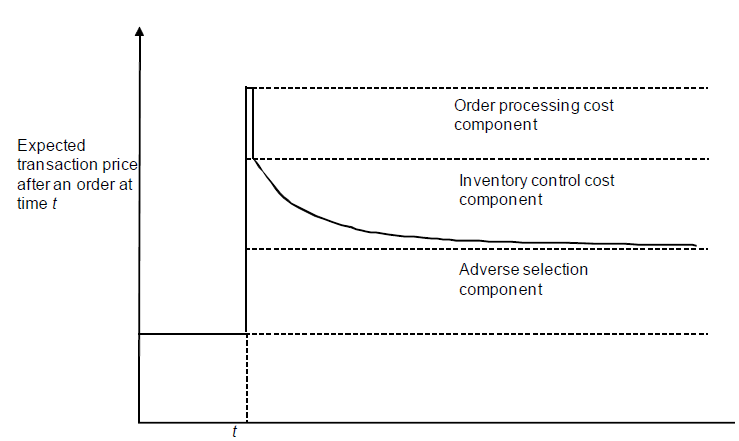
\includegraphics[width=0.8\linewidth]{pics/PriceDiscovery_Image}
\end{frame}


\begin{frame}{Measured price impact and the theories}
	\begin{itemize}
		\item Parameters of interest:
		\begin{itemize}
			\item $\gamma$: order-processing cost
			\item $\lambda$: price impact related to information
			\item $\beta$: price impact related to MM risk aversion
		\end{itemize}
		\item Data:
		\begin{itemize}
			\item Transaction prices $p_t$, net market order flow $q_t$, order sign $d_t$
		\end{itemize}
	\end{itemize}
\end{frame}


\begin{frame}{How to estimate?}
	\begin{itemize}
		\item Take GM model with order costs. There have:
		\begin{align*}
			p_t &= \mu_t + \gamma d_t
			\\
			\Rightarrow \varDelta p_t &= \mu_t - \mu_{t-1} + \gamma \varDelta d_t
		\end{align*}
		\item Further,
		\begin{align*}
			\mu_t = \mu_{t-1} + \lambda d_t + \varepsilon_t
		\end{align*}
		order flow is informative; also let $\varepsilon_t$ include all other kinds of public news
		\item Then
		\begin{align*}
			\varDelta p_t &= \lambda d_t + \gamma \varDelta d_t + \varepsilon_t
		\end{align*}
	\end{itemize}
\end{frame}


\begin{frame}{\cite{glosten_estimating_1988}}
	\begin{itemize}
		\item \textbf{\cite{glosten_estimating_1988}} estimate
		\begin{equation} \tag{5.7}
			\Delta p_t = \gamma_0 \Delta d_t+ \gamma_1 \Delta q_t + \lambda_0 d_t + \lambda_1 q_t + \epsilon_t
		\end{equation}
		jointly with trade directions $d_t$. 
		\item Accumulated order flow affects price level via $\lambda$, cyclical order flow gives $\gamma$ in the style of Roll's measure (2.15)
		\item On NYSE data from early 80s, they find $\gamma_1=\lambda_0=0$ and estimate $\gamma_0=.0465$, $\lambda_1=.0102$
	\end{itemize}
\end{frame}


\begin{frame}{Issues}
	\begin{itemize}
		\item Apart from the usual concerns with old empirical papers...
		\begin{itemize}
			\item not much data
			\item questionable specification
			\item questionable estimation procedures
		\end{itemize}
		\item ...there is the issue of ignoring inventory costs.
		\item In the short run, the effect of MM risk aversion would be similar
		\begin{equation} \tag{5.14}
		\Delta p_t = \gamma \Delta d_t + (\lambda + \beta) q_t + \epsilon_t
		\end{equation}
		\begin{itemize}
			\item $\lambda$ and $\beta$ are not separately identified.
		\end{itemize}
	\end{itemize}
\end{frame}


\begin{frame}[label=extending]{Including inventory costs}
	\begin{itemize}
		\item \textbf{\cite{hasbrouck_trades_1988}}: order flow is auto-correlated, so part of the order is not `news' but only moves inventory
		\item \textbf{\cite{huang_components_1997}}: suggest
		\begin{equation}\tag{5.17}
		q_t = \phi q_{t-1} + \eta_t
		\end{equation}
		\item Then (5.14) is modified to \hyperlink{derivation}{\beamerbutton{Derivation}}
		\begin{equation} \tag{5.21}
		\Delta p_t = \gamma \Delta d_t + (\lambda+\beta)q_t - \lambda \phi q_{t-1} + \epsilon_t
		\end{equation}
		\item They estimate the model for 20 major NYSE stocks: 
		\begin{align*}
			\phi &= -0.74	& \lambda &= 9.59\% S
			\\
			\beta &= 28.65\% S	& \gamma &= 61.76\% S
		\end{align*}
		%NOTE: negative phi makes sense with inventory costs
		\item Also: greater $\beta$ for larger transactions
	\end{itemize}
\end{frame}


\begin{frame}{Including inventory costs (2)}
		\begin{itemize}
			\item \textbf{\citet*{madhavan_why_1997}} find that $\lambda$ is higher in the morning, and $\gamma$ higher in the afternoon
			% more adverse selection in the morning; higher bargaining power for dealers at closing (traders want to unwind positions)
			\begin{itemize}
				\item Morning trading reveals all the information accumulated during off-market hours. Evening trading driven by traders' desire to close open positions
				\item \textbf{\cite{bogousslavsky_should_2020}}: closing auctions account for $7.3\%$ of daily trading volume, but contribute nothing to price discovery. Closing prices deviate a lot from midquotes, but revert back quickly.
			\end{itemize}
			\item \textbf{\cite{lyons_tests_1995}} had data on a FOREX dealer's inventory, and found $\beta$ very large
		\end{itemize}
\end{frame}


\begin{frame}{Long-run impact}
	\begin{itemize}
		\item Different dynamic approach: \textbf{\cite{hasbrouck_measuring_1991}} uses the long-run impact of an order $q_{t+1}$ on prices $p_{t+T}-p_t$ to identify the informational part of the trade
		\begin{itemize}
			\item The `impulse response' of prices to orders
			\item Opens door to richer time series analysis of transactions data
		\end{itemize}
		\item Findings: short-run effect of a trade $\approx 2\%$
		\item long-run effect of a trade ($T=5$ trades) $\approx 1\%$
		\begin{itemize}
			\item greater LR impact for stocks with lower capitalization
		\end{itemize}
	\end{itemize}
\end{frame}


\begin{frame}{Probability of Informed Trading}
	\begin{itemize}
		\item \textbf{\citet*{easley_liquidity_1996}}: use GM type model to estimate the prob. of informed trading
		\item On any given trading day, w.p. $\alpha$ there is some information event
		\begin{itemize}
			\item good or bad
			\item observed by informed traders, not by dealer
		\end{itemize}
		\item Within the day, \{informed traders, uninformed sellers, uninformed buyers\} arrive as Poisson process with intensity $\{\epsilon_i, \epsilon_s, \epsilon_b \}$
		\begin{itemize}
			\item Probability of observing $n$ traders of a particular type over the trading day is
			\[
			e^{-\epsilon} \frac{\epsilon^n}{n!}
			\]
		\end{itemize}
	\end{itemize}
\end{frame}


\begin{frame}{Probability of Informed Trading}
	\begin{itemize}
		\item Data for the number of buys and sells allow for estimation of these parameters with \structure{maximum likelihood}
		\item \textbf{\citet*{easley_is_2002}} estimate the `probability of informed trading' associated with any given order
		\begin{equation} \tag{5.27}
		PIN = \frac{\alpha \epsilon_i}{\epsilon_b + \epsilon_s + \alpha \epsilon_i}
		\end{equation}
		\item In NYSE data from 1983 to 1998:
		\begin{itemize}
			\item median PIN $=19\%$
			\item for $90\%$ of stocks, PIN is between $10\%$ and $30\%$
			\item greater for small-cap stocks, positively correlated with spread and price volatility
		\end{itemize}
		\item \textbf{\citet*{grammig_knowing_2001}} show that PIN is higher when markets are more anonymous
	\end{itemize}
\end{frame}


\begin{frame}{Conclusion}
	\begin{itemize}
		\item Depth of a market is closely tied to liquidity and is determined by most of the same factors
		\begin{itemize}
			\item Kyle model helps us analyze market depth, can accomodate all factors simultaneously 
			\item (except order costs)
			\item (we looked at version with only adverse selection -- see textbook for other versions)
		\end{itemize}
		\item Using the insights from last lecture we can estimate the importance of different components of the spread
		\begin{itemize}
			\item Perhaps surprisingly, order costs are by far the largest cost (but estimated on major stocks)
			\item Adverse selection is more of an issue in small-cap stocks
			\item \cite{easley_is_2002}: around 19\% of trading is informed
		\end{itemize}
	\end{itemize}
\end{frame}


\begin{frame}{Exercise}
\begin{itemize}
	\item for next Wednesday:
	\begin{itemize}
%		\item I uploaded two articles from the Economist, March 7, 2014, both on potential manipulation of prices
%		\item Consider these two issues:
%		\begin{itemize}
%			\item What motivates a trader to manipulate an asset's price? 
%			\item Is manipulation easier in a very liquid or a very illiquid market?
%		\end{itemize}
		\item Read the blog post on the story of how oil price came to be negative on April 20, 2020: \url{https://streetwiseprofessor.com/wti-wtf/}
	\end{itemize}
	\item for next Friday:
	\begin{itemize}
		\item solve exercise 3 in chapter 4 (p.159) which explores competition among speculators
	\end{itemize}
\end{itemize}
\end{frame}


\begin{frame}{Next week}
\begin{itemize}
	\item Analyze limit order markets: what is the difference to what we have done so far?
	\item Talk about the role of the `ticks', the priority rule, the interaction between dealers and LOBs, and a way to interpret limit orders
\end{itemize}
\end{frame}




\appendix
\begin{frame}[allowframebreaks]{References}
\bibliography{../teaching}
\bibliographystyle{abbrvnat}
\end{frame}



\begin{frame}[label=derivation, noframenumbering]{Derivation of (5.21)}
	Suppose $q_t=\phi q_{t-1}+\eta_{t}$. 
	\begin{itemize}
		\item \textbf{Adverse selection.} Notice that value equation is now
		\[
		\mu_t=\mu_{t-1}+\lambda[q_t-\mathbb{E}[q_t|\Omega_{t-1}]]+\epsilon_t.
		\]
		Only non-expected part of order flow carries information. 
		\item \textbf{Price.} The price equation then becomes
		\[
		p_t=m_t+\beta q_t+\lambda[q_t-\mathbb{E}[q_t|\Omega_{t-1}]]+\gamma d_t,
		\]
		where $m_t=\mu_t-\beta z_t$ is the `mid-price' from the Stoll model 
	\end{itemize}
\end{frame}


\begin{frame}[noframenumbering]{Derivation of (5.21)}
	\begin{itemize}
		\item Use $q_t=\phi q_{t-1}+\eta_{t}$ to get $\mathbb{E}[q_t|\Omega_{t-1}]=\phi q_{t-1}$.
		\item Take first differences of price equation
		\[
		\Delta p_t = \Delta m_t + \lambda [ \Delta q_t-\phi\Delta q_{t-1}]+\beta \Delta q_t+\gamma \Delta d_t
		\]
		\item Notice that $\Delta z_t=-q_{t-1}$ from market clearing condition. Then
		\[
		\Delta m_t = \Delta \mu_t-\beta \Delta z_t = (\lambda+\beta)q_{t-1}-\lambda \phi q_{t-2}+\epsilon_t.
		\]
		\item Substitute in to get
		\[
		\Delta p_t =(\lambda+\beta)q_{t-1} - \lambda\phi  q_{t-1}+\gamma \Delta d_t+\epsilon_t.
		\]
		\hyperlink{extending}{\beamerbutton{Back}}
	\end{itemize}
\end{frame}


\end{document} 